\chapter{Analysis}

Now that we have described the game's design, in this chapter, we will explain the approach we took to implement it from a high-level perspective.
We will provide concrete details only for what will be implemented in the playable demo version, but as always, we will make many decisions based on the original vision of our game.

\section{Game Engine}

Game engines provide many important and useful systems for us, so we can focus on implementing the game logic.
For our game, we chose Unity because it offers all the features we need, and the author is already familiar with it.
There are many game engines we could have used, and the high-level decisions presented in this chapter would be still applicable.
However, in some sections we will use nomenclature that is specific to Unity, so we assume the reader is at least familiar with it.
More information is available in the official documentation~\cite{UnityDocs}.

\section{Procedural Generation}

As explained in the previous chapter, a lot of the game will be procedurally generated including the map of a run and each battle along the way.
In the next few sections, we will decide how to generate the worlds for the battles, and in section~\ref{sec:analysis-waves}, we will focus on generating the waves of attackers.
The worlds are composed of three somewhat distinct parts~--- paths, terrain and obstacles.
It would make the most sense to generate each part separately, one after another.
We should start with the part that is most restricted, because each part is additionally restricted by what was generated before it.
For this reason, we will start with paths.
There is a lot of rules the paths should follow, as described in section~\ref{sec:design-paths}.
Additionally, the number of paths and their lengths heavily influence the difficulty of the battle.
A battle's difficulty should be decided by its position in the run, and it should be known to the player even before they select it, so they can decide which battle to fight.
So, we will generate paths first (section~\ref{sec:analysis-path-generation}), then the terrain (\ref{sec:analysis-terrain-generation}), and finally, the obstacles (\ref{sec:analysis-obstacles}).

From the player's perspective, all procedural generation and the rewards they receive will be random and unpredictable.
However, each run will have a single seed that deterministically decides all the \enquote{random decisions} the game makes.
Two runs with the same seed should look identical and if the player makes the same decisions and choices, the outcomes should be the same.
This allows the players to share seeds of the runs they found interesting and compare their skill in the same situations.
Furthermore, this is helpful for debugging, because it lets us easily reproduce any issue with the generation just by running it with the same seed.
As discussed in section~\ref{sec:design-saving}, we want to allow the player to save the game.
Here, determinism is also useful, because it allows us to save just the seed of the world that was generated, instead of saving it whole, which leads to simpler and smaller save files.

\subsection{Random Number Generators}

Randomized algorithms, like the ones we will use for procedural generation, depend on a \emph{random number generator} as their source of randomness.
A \textbf{random number generator} (or \emph{RNG}) produces a sequence of numbers that looks random and is unpredictable.
They are well explained in \citetitle{johnston2018random}~\cite{johnston2018random} by David Johnston.
Some RNGs use specialized hardware to generate truly random data using an external source of entropy, these are called \emph{true random number generators}.
However, we want a \emph{deterministic RNG}, also known as a \emph{pseudorandom number generator} (\emph{PRNG}).
These produce the random data using a completely deterministic algorithm, but unless we know the current internal state of the generator, the outputs still can't be predicted.
The initial state of a PRNG is called the \emph{seed}, and a generator will always generate the same sequence of outputs when \emph{seeded} with the same value.

Each query advances the generator's state, so the value a deterministic random number generator returns depends on the number of previous requests.
If we used one generator for generating everything, the outcomes of different systems would depend on the order they were generated in.
For example, when a player triggers some effect that uses randomness \emph{before} generating a level, the level would be different than if the player triggered the randomized effect \emph{after} the level was generated.
To remedy this, we will utilize a simple trick we call \emph{seed branching} all throughout the procedural generation.
Whenever we want more systems to be independent of each other, we create a new RNG instance for each system, and we seed them with each with a seed generated from the old RNG in advance.
For example, we will have a master RNG seeded with the seed of the run, from which we will generate the seeds for the map generator, reward systems, etc.
The map generator itself will generate the run map and then assign a new seed to each of the levels planned on the map, and so on.

We can determine what properties are required of the RNG we are going to use from our use-case.
First, obviously, the numbers generated by the generator should be random enough.
However, the RNG doesn't have to be cryptographically secure or pass strict statistical tests, since we aren't going to use them for cryptography or scientific simulations.
Since we will create many instances of the RNG, it should be lightweight and fast to initialize.
Some of them, for example the ones used by the reward system, will persist throughout the whole run, so we need an easy way to save the RNG's current state.
So, what options do we have?

Since we are using Unity, the first RNG that comes to mind is Unity class \mono{Random}~\cite{UnityRandom}.
It is designed to be easy to use, but it is very limited~--- for example, we have access to only one instance of the class and the same instance is used for other systems within the game engine.
This is a dealbreaker for us, because we want to create more instances, and we want to have complete control over them to ensure determinism.

Another option that's on-hand is .NET \mono{System.Random}~\cite{SystemRandom}.
According to the documentation, instantiating a random number generator is fairly expensive.
Furthermore, there are no methods to read and set the internal state of the generator.
This becomes a problem when we want to save the state of an instance to restore it later, for example when loading a save file.
We would have to serialize and deserialize the instance, which isn't a big problem, but it feels inelegant and inefficient.

Instead, we chose to go with a more straight-forward option~--- making our own RNG.
This way, we can make the generator have all the features we need.
There are many algorithms a PRNG can use.
Johnston describes in their book~\cite{johnston2018random} some most commonly used non-cryptographic PRNGs, namely:
\begin{itemize}
    \item Linear congruential generators (LCG),
    \item Multiply with carry (MWC),
    \item XORSHIFT,
    \item Permuted congruential generators (PCG).
\end{itemize}
All of these are random enough for our use-case, provided we use the right parameter values, so we chose an LCG, because it seemed the most simple to implement.
In the article \citetitle{LCGTables}~\cite{LCGTables}, the author explains the statistical tests they used to measure the randomness of the LCGs and tabulates the best-performing parameter combinations.
From there we took the parameters for our LCG implementation.

\section{Path Generation}\label{sec:analysis-path-generation}

In the previous section, we decided that when generating a world, we will start with the paths.
In section~\ref{sec:design-paths}, we outlined many requirements and suggestions for the paths, in order to make them play well.
We also mentioned that we will get the number of paths and their lengths as an input, because these values heavily influence difficulty.
However, there is still a lot of variance left for the player to deal with.
For example, the shape of the path can still vary a lot, not to mention the terrain and obstacles that will be generated after.

We should consider how is the difficulty influenced by the paths splitting into more branches or joining together.
When one path splits into two branches that go in separate directions, the battle should play out similarly to a battle with two distinct paths.
However, for the player, branching paths are not as difficult to manage as distinct paths.
They are usually closer together, because they have in common both the end point and the start point.
Furthermore, there is a stretch of path before it split into two branches, and a few tiles after the split, the branches are still pretty close together.
The player can concentrate their defenses around this portion of the level, partially mitigating the disadvantages of the split.

It is really hard to quantify the difficulty of more complex path networks.
However, we believe that the splits and joins do not influence the difficulty so much, that a greater control over them is required.
Especially with all the other sources of variance.

We can split the path generation process into three stages:
\begin{enumerate}
    \item Select sufficiently spaced out positions for the path starts, in order to spread the individual paths apart as much as possible.
    \item Generate the main branch of each path.
    \item Refine the paths in order to make them split into branches and join together.
\end{enumerate}
This is useful, because we can approach the path generation as three separate problems.
How to accomplish the goal of each of these stages will be described in the following subsections of this section.

\subsection{Path Starts}

In the first stage of path generation, we need to pick the path start positions.
As an input, we only get the Hub position, the number of paths, and their lengths.
Each path start must be at a position, such that a path of the given length can go from it to the Hub.

From the specification in section~\ref{sec:design-paths}, we know that paths must start just outside the world.
However, other segments of the paths are confined to the actual tiles of the world.
For simplicity, we will pretend from now on, that the paths start at an edge tile of the world, and add one segment going over the edge only after the paths are generated.
This segment is uniquely determined anyway, except in the corners of the world, where we can just always select the one that makes the path go straight, as shown in figure~\ref{fig:real-path-starts}.

\begin{center}
    \captionsetup{type=figure}
    \includegraphics[width=0.5\textwidth]{img/Real path starts.pdf}
    \caption{The red circles are the path starts we work with to stay within the bounds of the world. The blue arrows represent the first segment of each path that will only get added after the rest of the path was generated.}
    \label{fig:real-path-starts}
\end{center}

For a valid path of the correct length to exist between the Hub and the start, the start cannot be further from the Hub using \emph{Manhattan distance} that the path length.
Additionally, the Manhattan distance must have the same parity as the path length, i.e. a path with odd length must start an odd Manhattan distance from the Hub.
This is easy to see when we go along a path from the Hub to its start.
At the Hub, both Manhattan distance and \emph{path distance} are 0.
Whenever we go to the next tile, the path distance increases by 1, changing its parity.
The Manhattan distance can only increase by 1 or decrease by 1, also changing its parity.
Thus, at every tile on the path, the parities of the path distance and Manhattan distance match, including the path start.

In levels with more paths, we want the path starts to be spread out from each other, in order to cover the world with paths more evenly.
We can set a minimum distance between the paths starts.
For levels with just one long path, we can also set a minimum distance from the Hub, so it starts further away from it and has more space to zigzag through the world.

To actually select the starts, we find all tiles along the edge of the world, and separate them into two sets~--- each for one parity.
Then we can simply use rejection sampling to pick starts that satisfy the conditions on the distances.
As long as the minimum distances between path starts and from the \emph{Hub} are small enough, this approach always yields a valid collection of path starts.
However, with stricter parameters it is possible that the first few starts invalidate all other start positions.
In that case we can use rejection sampling again~--- trying to randomly select collections of starts, until we get one that's valid.
If the failure rate is great enough, it is wise to select a different algorithm, but our requirements are not very strict, so rejection sampling is fine.

\subsection{Generating the Main Paths}

From the previous step, we have a path start position for each path, in addition to the required lengths and hub position.
There is also a lot of rules for the paths, which we set in section~\ref{sec:design-paths}.

We couldn't find many resources on procedurally generated paths.
There is a lot of research on generating road networks, mazes or dungeons.
Theoretically, we could use one of the many algorithms for generating mazes~\cite{MazeWiki}, and modify it to suit our needs.
However, it would be difficult to achieve what we need using an approach that was designed for something else.

We found one algorithm specifically designed for procedurally generating paths, called \emph{path chiseling} by Boris the Brave on his blog~\cite{PathChiseling1}\cite{PathChiseling2}.
This algorithm creates random paths on a tile grid by randomly blocking off individual tiles until only one path remains.
This is more promising, however we were unable to find a good way to modify it to generate paths of specific lengths with the properties we want.

Since many of our requirements are more like suggestions, we always want to fulfill them almost the best we can.
This means we can look at the task as an optimization problem: create the \emph{best looking} paths, given the requirements like length, no crossing etc.
Since we want the paths to be randomized, we don't need to find the optimum, we only need a random solution that is good enough.
Given this, we decided to generate the paths using an optimization technique called \emph{simulated annealing}.

\subsection{Simulated Annealing}\label{sec:analysis-simulated-annealing}


A great analysis of this technique can be found in the article \citetitle{SimulatedAnnealing}~\cite{SimulatedAnnealing}.
In this section, we will describe the technique, and use it to generate the random paths we want.

Simulated annealing can be used to find an approximation of the global optimum much faster than it would take to find the exact global optimum.
The problems it can be used on have to be formulated as follows:
From the set of all states $S$, find a state $s^*$ that minimizes the cost function $f \colon S \to \R$, given a neighbor function $n \colon S \to \mathcal{P}(S)$ which gives the \emph{neighbor states} of each state.
For example, to use simulated annealing to solve the \emph{travelling salesman problem}, each state is usually defined as a permutation of the cities to be visited.
The cost function then gives the length of the salesman's path, and the neighbor function gives all the states that can be acquired by swapping two cities in the original state.

The process of simulated annealing is described in pseudocode in algorithm~\ref{alg:simulated-annealing}.
It starts in an initial state $s_0$ and runs for $max\_steps$ steps.
For each step, a temperature $t$ is computed, slowly decreasing from $t_{initial}$ in the first step, to $t_{final}$ at the final step.
In each step, a random neighbor $s'$ of the current state $s$ is selected, and an acceptance probability $p$ is computed, based on the values of $f(s)$, $f(s')$ and the current temperature $t$.
The new state $s'$ is then set as the current state with probability $p$.
This acceptance probability function always accepts a better new state ($s'$ such that $f(s') < f(s)$), but it can also give a non-zero probability when the new state is worse that the current state ($f(s') > f(s)$).
How often a worse state is accepted depends on the temperature.
At high temperatures, almost any state is accepted, at temperatures near zero, worse states are accepted very rarely.
Overall, the algorithm explores widely different states at the start, but settles into a local minimum over time, which is hopefully a global minimum thanks to the exploration at the start.

\begin{algorithm}[H]
    \caption{Simulated annealing}
    \label{alg:simulated-annealing}
    \begin{algorithmic}[1]
        \State $s \gets s_0$
        \For{$k$ from $0$ to $max\_steps-1$}
        \State $t \gets$ \Call{Lerp}{$t_{initial}$, $t_{final}$, $k/(max\_steps-1)$}
        \State $s' \gets$ random neighbor from $n(s)$
        \State $p \gets$ \Call{AcceptanceProbability}{$f(s)$, $f(s')$, $t$}
        \State with probability $p$: $s \gets s'$
        \EndFor\\
        \Return $s$
        \Statex
    \end{algorithmic}
\end{algorithm}

\subsection*{States}
To generate paths using simulated annealing, we need to define what is a state, a cost function and a neighbor function.
Each state will be a path network, where each path is a sequence of nodes.
Each node has a tile position, and each tile can contain multiple nodes.
Two consecutive nodes must be on neighboring tiles.
Additionally, each path starts at the given path start, has the given length, and ends at the tile with the \emph{Hub}.
Since we are going to change the paths only by a small amount at every step, we chose not to check for intersections.
Otherwise, we would lose too much freedom during the simulated annealing, and the final state would always end up close to the initial state.

\subsection*{Neighbor States}
The neighbors of a state are the states we obtain by changing the position of single node to a different position, such that the result is still a valid state.
This set is not too difficult to generate.
First, we can notice that the first and last node of every path can never change position.
Additionally, any node can only ever change its position to one other position, because it has to stay exactly 1 tile away from the nodes that come immediately before and after it.
This is shown in figure~\ref{fig:path-node-swaps}.
We only draw the nodes before and after the node which we want to modify, because the other nodes are not relevant.
As we can see, the new configuration is always obtained by switching the order of the two consecutive steps the path takes.
For example, in the first situation, the path changes from going down and left to going left and down.

\begin{center}
    \captionsetup{type=figure}
    \begin{tikzpicture}
        \draw[step=1.0,black,thin,shift={(0,0.5)}] (0,0) grid (2,2);
        \draw[step=1.0,black,thin,shift={(0,0.5)}] (4,0) grid (6,2);
        \draw[step=1.0,black,thin] (8,0) grid (9,3);
        \draw[step=1.0,black,thin] (11,0) grid (12,3);
        \begin{scope}[blue,very thick,decoration={
                        markings,
                        mark=between positions 0.25cm and -0.15cm step 0.5cm with {\arrow{>}};
                    }]
            \draw[postaction={decorate},shift={(0.5,1)}] (0,1)--(0,0)--(1,0);
            \draw[postaction={decorate},shift={(0.5,1)}] (4,1)--(5,1)--(5,0);
        \end{scope}
        \begin{scope}[blue,very thick,decoration={
                        markings,
                        mark=between positions 0.3cm and -0.15cm step 0.5cm with {\arrow{>}};
                    }]
            \draw[postaction={decorate},shift={(0.5,0.5)}] (7.8,1)--(8,2);
            \draw[postaction={decorate},shift={(0.5,0.5)}] (8,2)--(8.2,1);
            \draw[postaction={decorate},shift={(0.5,0.5)}] (10.8,1)--(11,0);
            \draw[postaction={decorate},shift={(0.5,0.5)}] (11,0)--(11.2,1);
        \end{scope}
        \filldraw[black,shift={(0.5,1)}] (0,1) circle (3pt);
        \filldraw[red,shift={(0.5,1)}] (0,0) circle (3pt);
        \filldraw[black,shift={(0.5,1)}] (1,0) circle (3pt);
        \filldraw[black,shift={(0.5,1)}] (4,1) circle (3pt);
        \filldraw[red,shift={(0.5,1)}] (5,1) circle (3pt);
        \filldraw[black,shift={(0.5,1)}] (5,0) circle (3pt);
        \draw[->,very thick,shift={(0.5,0.5)}] (2,1) -- (3,1);
        \filldraw[black,shift={(0.5,0.5)}] (7.8,1) circle (3pt);
        \filldraw[red,shift={(0.5,0.5)}] (8,2) circle (3pt);
        \filldraw[black,shift={(0.5,0.5)}] (8.2,1) circle (3pt);
        \filldraw[black,shift={(0.5,0.5)}] (10.8,1) circle (3pt);
        \filldraw[red,shift={(0.5,0.5)}] (11,0) circle (3pt);
        \filldraw[black,shift={(0.5,0.5)}] (11.2,1) circle (3pt);
        \draw[->,very thick,shift={(0.5,0.5)}] (9,1) -- (10,1);
    \end{tikzpicture}
    \caption{Possible node position changes to create a neighbor state.}
    \label{fig:path-node-swaps}
\end{center}

\subsection*{Cost Function}
Now we select a cost function that gives a better score to paths that are more desirable.
Since we want the paths to spread out, we can calculate fore each tile what we call a \emph{crowding penalty}.
Each node contributes 1 crowding to the tile it's on, and all other tiles get a lower penalty decreasing with distance.
In the end we chose the following formula for the crowding penalty $c$ of a tile $t$ caused by a path node on tile $n$:
\begin{equation*}
    c = \frac{1}{\abs{t - n}^4 + 1}
\end{equation*}
Each tile's total crowding penalty is the sum of the contribution from each node.
We raise the distance to the power of 4, because in our testing, lower exponents led to paths influencing each other from too far away.

We also add a big crowding penalty to the tiles along the edge of the world, which gradually decreases as we go away from the edge.
This is to push the paths away from the edges, as this is undesirable for reasons specified in section~\ref{sec:design-paths}.

We could then calculate the cost function of a state as the sum of the crowding penalties of each tile for each node on it.
However, to save on computation, we don't actually compare the values of the current and next state.
Instead, we only calculate the \emph{relative improvement} of the position change as $crowding($crurrent position$) - crowding($future position$)$ without even calculating the new crowding penalties.
We only recalculate the crowding penalties for a state after we select it as the new state.
This is only a very crude approximation of the real relative improvement $f(s) - f(s')$, and it is biased towards changing the node's position, because the current position has greater crowding penalty from the node itself, while the future position is not affected as much.
Later, we will show how we changed the algorithm to mitigate this bias.

\subsection*{Initial State}
All that's left is to produce an initial state.
This is not trivial, because of our constraints on what's considered a valid state.
Namely, every path has to be the correct length.
However, we can easily produce a valid initial state using a random walk from each path start.
For each path, the algorithm starts on the path start tile, and create the first path node.
Then it repeatedly moves its current position to a random neighbor of the current tile, and places the next path node there.
This is repeated until it creates a path of the correct length.
However, we need to ensure that the path ends at the Hub.
To achieve this, we just make the algorithm never select a tile that is further away from the Hub (in Manhattan distance), than the remaining length of the path.

\subsection*{Modified Algorithm}
We used a slightly different version of the algorithm, as seen in algorithm~\ref{alg:annealing-paths}.
The first difference from algorithm~\ref{alg:simulated-annealing} is that at each step we don't pick a random candidate, and then switch to it with some probability.
This would lead to a lot of steps, where we don't change the state.
We skip all those steps, by instead calculating a weight for each of the candidates, giving greater weight to better candidates.
Then we select a random one, weighted by these weights, and always switch to it.
For some candidates, the weight comes out as less than or equal to 0, and we don't add it to our list of candidates.
This is the same as if the candidate had an acceptance probability of 0.

Another change we make is to calculate an approximation of the relative improvement $f(s) - f(s')$, instead of calculating $f(s)$ and $f(s')$ separately.
This is to save on computation, as described before.
However, we also immediately add the temperature to the relative improvement, in order to offset the bias our approximation introduces.
We just change the temperature range to end at a negative value.
This value does not have to be exact, because the temperature changes, so it will always be too high or too low anyway.

\begin{algorithm}[H]
    \caption{Simulated annealing for generating paths}
    \label{alg:annealing-paths}
    \begin{algorithmic}[1]
        \State $s \gets$ \Call{GenerateInitialPaths}{}
        \State $crowding \gets$ \Call{CalculateCrowding}{$s$}
        \Statex
        \For{$k$ from $0$ to $max\_steps-1$}
        \State $t \gets$ \Call{Lerp}{$t_{initial}$, $t_{final}$, $k/(max\_steps-1)$}
        \Statex
        \State $candidates \gets \varnothing$
        \ForEach{node swap $x = a \to b$ in \Call{GetPossibleNodeSwaps}{$s$}}
        \State $improvement \gets crowding(a) - crowding(b) + t$
        \If{$improvement > 0$}
        \State $candidates \gets candidates + (x,\ improvement)$
        \EndIf
        \EndFor\\
        \State $x \gets$ random node swap from $candidates$ weighted by $improvement$
        \State $s \gets s$ with $x$ applied
        \State $crowding \gets$ \Call{UpdateCrowding}{$crowding$, $x$}
        \EndFor\\
        \Return $s$
        \Statex
    \end{algorithmic}
\end{algorithm}

\subsection*{Intersection Untwisting}
However, this algorithm still sometimes produces paths that intersect themselves.
This is because it is difficult for the algorithm to fix a loop in the path, as shown in figure~\ref{fig:untwisting-paths}.
It would first have to bring many nodes closer together, in order to let them cross over each other.
However, we can add a step that just \emph{untwists} crossings by reversing the section of the path that forms a loop, as shown in the figure.
This still leaves two nodes on the same tile, but annealing can drive these apart without any issue.

\begin{center}
    \captionsetup{type=figure}
    \begin{tikzpicture}
        \draw[step=1.0,black,thin] (0,0) grid (4,4);
        \draw[step=1.0,black,thin] (6,0) grid (10,4);
        \begin{scope}[blue,very thick,decoration={
                        markings,
                        mark=between positions 0.25cm and -0.05cm step 0.5cm with {\arrow{>}};
                    }]
            \draw[postaction={decorate},shift={(0.5,0.5)}] (-1,1)--(3,1);
            \draw[white,line width=4pt,shift={(0.5,0.5)}] (1,0.6)--(1,1.4);
            \draw[postaction={decorate},shift={(0.5,0.5)}] (3,1)--(3,3)--(1,3)--(1,-1);
            \draw[postaction={decorate},shift={(0.5,0.5)}] (5,1)--(6.95,1.05);
            \draw[postaction={decorate},shift={(0.5,0.5)}] (6.95,1.05)--(7,3);
            \draw[postaction={decorate},shift={(0.5,0.5)}] (7,3)--(9,3)--(9,1);
            \draw[postaction={decorate},shift={(0.5,0.5)}] (9,1)--(7.05,0.95);
            \draw[postaction={decorate},shift={(0.5,0.5)}] (7.05,0.95)--(7,-1);
        \end{scope}
        \draw[->,very thick,shift={(0.5,0.5)}] (4,1.5) -- (5,1.5);
    \end{tikzpicture}
    \caption{Untwisting a self-intersecting path.}
    \label{fig:untwisting-paths}
\end{center}

This is valid, because the length of the path doesn't change.
However, we cannot untwist crossings between two different paths, because that could change their lengths.
This means that we should take special care to not produce an initial state where two different paths cross.
We can achieve this by calculating crowding penalties when creating the initial state.
Then, when the algorithm selects a random neighbor to move to, we make it prefer the neighbors with a lower crowding penalty.
Because we don't mind self-intersections, we don't add the crowding penalties from the nodes of the path the algorithm is currently creating.
We add them only when the path is complete.

Sill, the algorithm sometimes fails in creating a valid path network.
In case no valid network is generated, we can restart the path generation algorithm, including picking the starting positions.

In figure~\ref{fig:simulated-annealing}, we can see how the paths evolve over time as the temperature decreases.
\begin{center}
    \captionsetup{type=figure}
    \begin{minipage}{.5\textwidth}
        \centering
        \includegraphics[width=0.95\linewidth]{img/SA initial state.pdf}
        \subcaption{Initial state ($t_{initial} = 2$)}
    \end{minipage}%
    \begin{minipage}{.5\textwidth}
        \centering
        \includegraphics[width=0.95\linewidth]{img/SA temp 1.5.pdf}
        \subcaption{$t = 1.5$}
    \end{minipage}\\
    \begin{minipage}{.5\textwidth}
        \centering
        \includegraphics[width=0.95\linewidth]{img/SA temp 0.5.pdf}
        \subcaption{$t = 0.5$}
    \end{minipage}%
    \begin{minipage}{.5\textwidth}
        \centering
        \includegraphics[width=0.95\linewidth]{img/SA final.pdf}
        \subcaption{Result ($t_{final} = -0.5$)}
    \end{minipage}
    \caption{Evolution of paths during simulated annealing.}
    \label{fig:simulated-annealing}
\end{center}

\subsection{Final Paths}

Now that we have generated the main paths, we just have to generate the side branches.
Again, we could use some randomized algorithm.
We don't want the branching to feel the same in every level, so we would need to come up with complicated heuristics to ensure the paths we generate vary a lot.
The world generation steps that come after have to make sure to not block the paths we have generated, but we don't want to constrain it with the side branches too.

Since we don't have any requirements on the side branch count or their lengths, we can use a much simpler solution.
We can generate the rest of the world first, and only then make extra paths where they fit.
This also leverages the randomness of the world generation instead of needing to introduce more on our own.

This means, that this step will start with an already generated terrain and obstacles, as described in sections~\ref{sec:analysis-terrain-generation} and~\ref{sec:analysis-obstacles}.
These steps respect the original paths, but they will cause other tiles or edges between them to be blocked, as shown in figure~\ref{fig:paths-world}.
Here, we can see the original paths on the left.
On the right, we can see tiles blocked by obstacles as gray squares with black edges.
Additionally, some edges between tiles are also blocked, usually because the two tiles are at different height levels, separated by a cliff.
These are the remaining black lines.

\begin{center}
    \captionsetup{type=figure}
    \begin{minipage}{.5\textwidth}
        \centering
        \includegraphics[width=0.95\textwidth]{img/Generated Paths.pdf}
    \end{minipage}%
    \begin{minipage}{.5\textwidth}
        \centering
        \includegraphics[width=0.95\textwidth]{img/Paths and world.pdf}
    \end{minipage}
    \caption{Blocked edges and tiles after generating the terrain and obstacles.}
    \label{fig:paths-world}
\end{center}

The rest of the world generation has made sure that at least the main paths are still traversable, however we don't have to adhere to them completely.
For example, we would like them to sometimes join together, which we cannot do without changing them.

There are so many blocked edges that we can just greedily add all the valid side branches we find.
To do this, we will use depth first search, but we will add a few heuristics to produce better paths.
To decide on these heuristics, we will set a few more requirements:
We still want the paths to be spread out, but we would also prefer the paths to go straight if possible.
Additionally, we can see there are some \emph{choke points}~--- tiles, which have to have a path going through them, because all valid paths from one start go through them.

Each tile can only have one path distance from the Hub, as specified in section~\ref{sec:design-paths}.
We want these tiles to have the same path distance as the distance on the original path.
This heavily reduces the number of possible paths, while making sure, that the paths don't bunch up at the start or near the Hub, because it will make them keep a similar distribution to the originally generated paths.
We can see the choke points for the paths we generated in figure~\ref{fig:choke-points}.
They are shown as a blue circle with a number representing the path distance to the Hub.

Above all, we need to make sure the paths we produce are the correct length.
We can save a lot of time by precomputing the distance from each tile to the Hub, respecting all the blocked tiles and edges.
For this, we can do a breadth first search from the Hub tile.
However, we can also introduce the required distances for the choke points.
Finding the choke points is not trivial, so we instead set a minimum distance for every tile on one of the generated paths.
The result can be seen in figure~\ref{fig:path-distances}.

\begin{center}
    \begin{minipage}{.5\textwidth}
        \centering
        \captionsetup{type=figure,width=0.9\textwidth}
        \includegraphics[width=0.95\textwidth]{img/Path choke points.pdf}
        \caption{Path choke points and their respective distances.}
        \label{fig:choke-points}
    \end{minipage}%
    \begin{minipage}{.5\textwidth}
        \centering
        \captionsetup{type=figure,width=0.9\textwidth}
        \includegraphics[width=0.95\textwidth]{img/Path Distances.pdf}
        \caption{Minimum distances calculated in the first step.}
        \label{fig:path-distances}
    \end{minipage}
\end{center}

Now we finally run the depth first search, one path by one.
The algorithm keeps a stack of \emph{path prototypes}.
These are paths, which start at the start tile, but have not reached the Hub yet.
At the start, the stack contains only the path prototype with only the start position as its only element.
At every step, the algorithm pops the last prototype from the stack, finds all valid one-step continuations of the current paths, and adds those to the stack.

Valid continuations are tiles that can be reached from the last tile of the current path prototype in one step.
Additionally, they have to have a distance that is less than or equal to the remaining length of this path prototype.
The valid continuations are ordered such that the best option will be put onto the stack last, so it gets popped in the next step.
The best option is always the one that goes straight, and the rest is ordered by the crowding penalty of the tile, which is calculated similarly to section~\ref{sec:analysis-simulated-annealing}.

Once the algorithm reaches the \emph{Hub} or an already existing path, it checks whether it is valid to finish the current path.
First, it must have the correct remaining length to produce a valid path.
When it connects to the Hub, the remaining length must be 0, and for connecting to an existing path, the remaining length must match the path distance of that tile.
Additionally, as per the last rule in the summary of section~\ref{sec:design-paths}, every side branch must go through at least one tile that is not adjacent to any already existing path.

If this check fails, the algorithm does not mark this path, it pops the last item from the stack and continues from there.
If the check succeeds, it marks the new path section and updates the crowding penalties to take the new path section into account.
Then it continues by making another branch, this time taking an item from the opposite end of the stack.
This is done to minimize the length of path the new branch shares with the branch it came from.
The first item on the stack should have the least amount of path segments in common with the last item.
The entire search is described in pseudocode as algorithm~\ref{alg:path-finalizing}.

\begin{algorithm}[H]
    \caption{Finalizing paths}
    \label{alg:path-finalizing}
    \begin{algorithmic}[1]
        \ForEach{path start $start$}
        \State $stack$.\Call{PushLast}{path prototype containing only $start$}
        \State $success \gets$ \mono{false}
        \Statex
        \While{$stack$ is not empty}
        \If{$success$}
        \State $p \gets stack$.\Call{PopFirst}{}
        \Else
        \State $p \gets stack$.\Call{PopLast}{}
        \EndIf
        \Statex
        \If{last tile in $p$ contains a path or the Hub}
        \State $success \gets$ \Call{TryFinishPath}{$p$}
        \Else
        \State $success \gets$ \mono{false}
        \ForEach{tile $c$ from \Call{GetValidContinuations}{$p$}}
        \State $stack$.\Call{PushLast}{$p$ extended by $c$}
        \EndFor
        \EndIf
        \EndWhile
        \EndFor
        \Statex
    \end{algorithmic}
\end{algorithm}

However, there is one more optimization we can make.
With this ordering of valid continuations, the algorithm usually reaches the Hub too soon, and then it has to backtrack many times, before producing a path that is the right length.
To fix this, we prioritize above all the tiles with distance to the Hub exactly equal to the remaining length.

The results of the algorithm are displayed on the right in figure~\ref{fig:final-paths}, compared to the initially generated paths on the left.
Segments that have changed are highlighted in red.

\begin{center}
    \captionsetup{type=figure}
    \begin{minipage}{.5\textwidth}
        \centering
        \includegraphics[width=0.95\textwidth]{img/Paths and world.pdf}
    \end{minipage}%
    \begin{minipage}{.5\textwidth}
        \centering
        \includegraphics[width=0.95\textwidth]{img/Final Paths.pdf}
    \end{minipage}
    \caption{Final paths compared to the originally generated paths.}
    \label{fig:final-paths}
\end{center}

\section{Terrain Generation}\label{sec:analysis-terrain-generation}

There are many techniques we could use for generating the terrain.
However, we have pretty strict requirements for the terrain generation.
For example, we need to make sure the paths we have generated in the previous step are not blocked by terrain features like cliffs.

This led us to choose a variant of a procedural generation algorithm called \emph{model synthesis}, originally developed by \Citeauthor{ModelSynthesis}~\cite{ModelSynthesis}.
The discrete version of this algorithm is better known by the name \emph{wave function collapse} (or~WFC in short), popularized by \Citeauthor{WFC} on GitHub~\cite{WFC}.
Model synthesis is more general and focuses more on 3D models, whereas WFC applies the same concepts to generating 2D pixel art and tile maps.
Since the name \enquote{wave function collapse} is more popular, we will use it in the rest of this thesis, even though it's not the original name.

We chose WFC, because it can generate randomized terrain, whilst fully respecting the initial constraints we give it.
To see how this works, we will explain the algorithm first.

\subsection{Wave Function Collapse}

The original intent behind the algorithm is to replicate the structure of an example on a larger scale, making sure that the output is locally similar to the input, as shown in figure~\ref{fig:wfc-example}.
We will limit our examples to 2-dimensional grids of tiles, however this algorithm works in more dimensions, and even for irregular cells.

\begin{center}
    \captionsetup{type=figure}
    \includegraphics[width=0.5\textwidth]{img/WFC Example.pdf}
    \caption{Example input and output of the wave function collapse algorithm.}
    \label{fig:wfc-example}
\end{center}

The first step of the algorithm is to extract from the input which features can appear next to each other.
The algorithm creates a set of \emph{modules}\footnote{This is a naming convention used in an article by \Citeauthor{WFCMarian}~\cite{WFCMarian}.}, which are the building blocks the output will be built from.
Each module comes with a set of constraints on its neighbors.
The main portion of the algorithm then builds the output from these modules, such that all the constraints are satisfied, and each module appears in the output with a similar frequency to the input.
However, we will create the modules for our generator by hand, including their constraints, in order to have greater control over the generated result.
In figure~\ref{fig:wfc-modules}, we can see a set of 7 modules and the resulting output, given only the constraint that the edges of directly adjacent modules must match.

\begin{center}
    \captionsetup{type=figure}
    \includegraphics[width=0.5\textwidth]{img/WFC modules.pdf}
    \caption{Example output of WFC, using the modules on the left and only the constraint that their edges must match.}
    \label{fig:wfc-modules}
\end{center}

We call each spot in the output where a module is supposed to be a \emph{slot}.
Each slot keeps track of all the modules that can be placed in it.
At the start of the main part of the algorithm, all slots are initialized with all the modules.
Figure~\ref{fig:wfc-initial} shows a visualization of this state.
Then the algorithm repeats two actions: collapse a slot, propagate constraints.
To collapse a slot, the algorithm removes all possible modules from the slot except for one, chosen at random.

Then it has to propagate constraints, which means that it removes from each slot all the modules which can no longer be placed there.
For example, in figure~\ref{fig:wfc-step-1} we see that a slot has collapsed to a module which has a line on each edge.
Thus, the algorithm removes from the neighboring slots (marked in red) all modules which don't have a line at the corresponding edge.
After propagating constraints, the algorithm collapses another slot and so on.

\begin{center}
    \captionsetup{type=figure}
    \begin{minipage}{.31\textwidth}
        \centering
        \includegraphics[width=0.95\linewidth]{img/WFC initial state.pdf}
        \subcaption{Initial state} \label{fig:wfc-initial}
    \end{minipage}%
    \begin{minipage}{.31\textwidth}
        \centering
        \includegraphics[width=0.95\linewidth]{img/WFC step 1.pdf}
        \subcaption{First step} \label{fig:wfc-step-1}
    \end{minipage}%
    \begin{minipage}{.31\textwidth}
        \centering
        \includegraphics[width=0.95\linewidth]{img/WFC step 2.pdf}
        \subcaption{Second step} \label{fig:wfc-step-2}
    \end{minipage}
    \caption{Two steps of wave function collapse. Uncollapsed slots are drawn in light blue, uncollapsed slots that changed are drawn in red.}
    \label{fig:wfc-steps}
\end{center}

In figure~\ref{fig:wfc-step-2}, we can see an interesting situation after collapsing a second slot.
The slot between the collapsed slots can still contain two possible modules, however both of them have a line at the top and bottom edges.
This means that the algorithm also has to propagate to the neighbors of this tile that they have to have lines at the corresponding edges.
A change in one slot can affect slots even very far away from it.

This process repeats until all slots are collapsed, at which point we have successfully generated the output.
This process is summarized as algorithm~\ref{alg:wfc}.
We left out one detail: which element does \textsc{Pop} select?
This does not matter for the overall function of the algorithm, and it will be further discussed in section~\ref{sec:analysis-our-wfc}.
We will call this algorithm WFC, even though it differs from both WFC by Gumin and Merrell's model synthesis.
The only notable difference is that we skip the feature extraction step, and the algorithm takes as input the modules directly.

\begin{algorithm}[H]
    \caption{A na\"{i}ve version of wave function collapse}
    \label{alg:wfc}
    \begin{algorithmic}[1]
        \ForEach{slot $s$ in output} \Comment{Initialize all slots.}
        \State $s.modules \gets all\_modules$
        \EndFor
        \Statex
        \State $uncollapsed \gets$ all slots
        \While{$uncollapsed$ is not empty}
        \State $s \gets uncollapsed$.\Call{Pop}{} \Comment{Collapse a slot.}
        \State $s.modules \gets \{$random module from $s.modules\}$
        \Statex
        \State $to\_update \gets$ neighbors of $s$ \Comment{Propagate constraints.}
        \While{$to\_update$ is not empty}
        \State $u \gets to\_update$.\Call{Pop}{}
        \Statex
        \State $changed \gets$ \mono{false}
        \ForEach{module $m$ in $u.modules$} \Comment{Remove invalid modules.}
        \If{not \Call{IsValid}{$m$}}
        \State $u.modules \gets u.modules - m$
        \State $changed \gets$ \mono{true}
        \EndIf
        \EndFor
        \Statex
        \If{$changed$} \Comment{If $u$ changed, enqueue its neighbors.}
        \State $to\_update \gets to\_update\,\cup$ neighbors of $u$
        \EndIf
        \Statex
        \EndWhile
        \EndWhile
        \Statex
    \end{algorithmic}
\end{algorithm}

However, it is possible for the algorithm to create a slot with no valid module.
In that case, it is no longer possible to create a valid output.
We call this situation a \emph{conflict}.
An example can be seen in figure~\ref{fig:wfc-backtracking}.
If we look at WFC as a \emph{constraint satisfaction problem} solver, we can see that the constraint propagation only ensures \emph{arc-consistency}, which is not enough to rule out conflicts~\cite{LocalConsistencyWiki}.

We called algorithm~\ref{alg:wfc} na\"{i}ve, because it is unable to deal with any conflicts.
What can we do to always produce a result, even when a conflict happens?
One option is to simply restart the algorithm.
For sufficiently small outputs, this should be rare enough, only needing a few restarts.

Another option is to use backtracking.
Whenever the algorithm runs into a contradiction after collapsing a slot, it returns to the state before collapsing.
Additionally, it removes the module the slot collapsed to from its valid options, because it now knows it causes to a conflict.
The state after backtracking is illustrated in fig~\ref{fig:wfc-after-backtracking}.
This way, the algorithm can continue generating without getting rid of all its progress.

\begin{center}
    \captionsetup{type=figure}
    \begin{minipage}{.31\textwidth}
        \centering
        \includegraphics[width=0.95\linewidth]{img/WFC backtracking before.pdf}
        \subcaption{Before collapsing} \label{fig:wfc-before-backtracking}
    \end{minipage}%
    \begin{minipage}{.31\textwidth}
        \centering
        \includegraphics[width=0.95\linewidth]{img/WFC backtracking dead end.pdf}
        \subcaption{After collapsing} \label{fig:wfc-dead-end}
    \end{minipage}%
    \begin{minipage}{.31\textwidth}
        \centering
        \includegraphics[width=0.95\linewidth]{img/WFC backtracking after.pdf}
        \subcaption{After backtracking} \label{fig:wfc-after-backtracking}
    \end{minipage}
    \caption{Conflicts and backtracking in WFC. The red cross marks a slot with no valid modules.}
    \label{fig:wfc-backtracking}
\end{center}

\subsection{Advantages and Disadvantages of WFC}

The main advantage of WFC is that it offers a lot of control over the generated world.
That's ultimately why we chose to use it.
We always know what features can appear in the world, because we explicitly allowed them to exist.
We can also freely constrain the world that we are generating.
For example, we can force the generator to not block the paths we've generated in the previous stage, and we can force the tile with the Hub to be flat.
We also force a random tile to be at the lowest height level and another to be at the highest.

However, WFC has some disadvantages when used as a terrain generator.
First, it can be very slow.
The time it takes algorithm~\ref{alg:wfc} to run scales linearly with the number of slots, which is not bad when we never run into contradictions.
Merrell shows in their thesis that deciding whether an incomplete output is consistent, i.e. it can be completed without running into contradictions, is an NP-complete problem.
This necessarily means that WFC isn't very fast in the worst case.

The real problem is that the algorithm usually does run into contradictions, and the larger the generation task, the more likely it is to run into a contradiction.
This is especially bad for online generation of infinite worlds, because we can't simply restart and generate a new world after the player has already seen a part of it.
Backtracking also doesn't solve this issue, because the algorithm can collapse a slot in a way that is guaranteed to cause a contradiction, and then do arbitrarily many more steps before finally running into it.
Of course, there are ways to circumvent this issue, namely by making the individual generation tasks smaller.
In their thesis, Merrell describes a technique called \emph{modifying in parts} based on this approach.

Another potential problem with WFC is that the individual slots or modules can be very apparent and repetitive.
This can be solved by procedurally generating the resulting geometry the player sees, only based on the modules chosen by WFC.
Another way to make the slots less apparent is to make the slots irregular.
Both of these techniques are used by \emph{Townscaper}~\cite{Townscaper}, a game by Oskar St\r{a}lberg.

Also, WFC only uses local constraints, so it provides no control over the more global features of the output.
On a large scale, the results are very homogenous.
For larger outputs, WFC should only be used to generate the local features, guided by large-scale features generated by some other algorithm.

Luckily, none of these disadvantages matter for our use case.
Our worlds are very small, and we don't mind that the tiles will be apparent, since the gameplay of our game is centered around them anyway.

\subsection{Using WFC for Terrain Generation}\label{sec:analysis-our-wfc}

Even though we want to generate a 3D terrain, our output will consist of a 2D grid of slots.
We want the tiles of the generated world to be at different heights, however, we don't want any tiles to generate above other tiles.
Ultimately, this is a 2D generation task, with the addition that modules can appear at different height levels.

At first, it might seem sensible to have one slot per world tile.
However, each tiles on it sown will be mostly a flat square.
The interesting terrain features will appear on the boundaries between the tiles.
For example, two tiles at different height levels next to each other will have a cliff separating them.
If we wanted to incorporate the cliff into the tile module, which tile does it belong to?
What about the features where the corners of four tiles meet?
We offset the slots in a way shown in figure~\ref{fig:tiles-and-slots}, such that each slot is responsible for four quarter-tiles of the world.
This way, the modules dictate how can the adjacent tiles connect to each other.

\begin{center}
    \captionsetup{type=figure}
    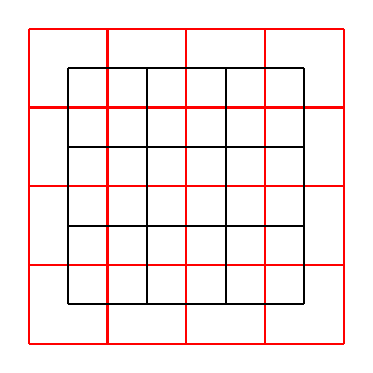
\begin{tikzpicture}
        \draw[step=1.0,thick,red] (0,0) grid (4,4);
        \draw[step=1.0,black,thick,shift={(0.5,0.5)}] (0,0) grid (3,3);
    \end{tikzpicture}
    \caption{The slots for generating a $3\times3$ tile world. Tiles are drawn in black, slots in red.}
    \label{fig:tiles-and-slots}
\end{center}

One example of such module is shown in figure~\ref{fig:wfc-module}.
Each module constrains the 8 adjacent slots.
An edge type is specified for each edge, and modules which share an edge must have the same edge type.
For each corner of the module, several tile constraints are specified.
The modules that share a tile must agree on the tile's properties: its height, slant direction (if any) and surface type.
Terrain types can have multiple surface types, each with a different set of modules and a few modules that allow to transition between them.
For example, a \emph{shore} module could have \emph{ground} tiles on one side and \emph{water} tiles on the other.
For each terrain type, it is also specified which surface types and which edge types block paths.

\begin{center}
    \captionsetup{type=figure}
    \begin{minipage}{.5\textwidth}
        \centering
        \includegraphics[width=0.95\textwidth]{img/Module model.png}
    \end{minipage}%
    \begin{minipage}{.5\textwidth}
        \centering
        \includegraphics[width=0.95\textwidth]{img/Module constraints.pdf}
    \end{minipage}
    \caption{An example module and its constraints.}
    \label{fig:wfc-module}
\end{center}

In figure~\ref{fig:wfc-modules}, we show 7 modules as an input.
However, when designing them, it would make more sense to think of them as 3 different modules that can each be rotated.
Thus, the modules we use will also have an option to select the allowed reflection and rotations.
Then, before generating the terrain, we will automatically generate all variants of each module.
Each module can also be placed at different height levels, which is handled similarly.
For example, the module shown in figure~\ref{fig:wfc-module} will effectively become 24 different modules in a terrain type with 4 height levels (0, 1, 2, 3), because it has 8 different reflections and rotations, and it can appear at 3 different height levels (0--1, 1--2, 2--3).

For each module, we also specify a weight.
This dictates how likely it is to be selected when collapsing a slot, compared to other modules.
For example, when we collapse a slot that only has two valid modules, with weights 1 and 4, then the first module will be selected with a 20\,\% probability.

We have decided to implement backtracking to solve contradictions.
If the algorithm only ever has to backtrack once before collapsing another slot, we say that it needs backtracking depth 1.
However, it is possible that the algorithm collapses a slot, finds a contradiction, and after backtracking, removes the only remaining module in the slot that was collapsed.
Thus, it creates another contradiction, which causes it to backtrack deeper.
We run some quick tests with the set of modules which is going to be used to generate terrain in the demo version.
During these tests, we were unable to generate a single world, without running into a contradiction.
However, most worlds only ever needed backtracking depth of 1 to successfully generate.
After that, we ran into diminishing returns.
Of the worlds that required backtracking depth 2, most required backtracking depth greater than 10.
So we decided to allow for backtracking depth 1 and otherwise just restart the generation, which makes it faster on average.

\xxx{I should probably provide the exact data I measured. Do I also need to explain the whole setup to make it reproducible?}

We also need to decide which slot to collapse at each step of the algorithm.
Merrell uses in their thesis a sort of scan line order, collapsing them in the lexicographic order of their coordinates.
This could theoretically introduce a directional bias in the results.
Gumin in their implementation always collapses a slot with the lowest \emph{Shannon entropy}.
This causes the generation to collapse slots outwards form the slot that was collapsed first.
From our testing, the results tend to look unnatural, often creating rectangular regions at the same height, or repeating patterns.

Both of these orders grow the collapsed portion of the world from one initial slot, similar to growing a regular crystal from one seed crystal.
To make the results more natural, we chose to select the slot to collapse at random.
This leads to the generator first collapsing slots in various parts of the world to different configurations.
Then it has to somehow connect these to make the world follow the rules we set.
This leads to more diverse results, however, the failure rate becomes very high, leading to slower generation.

As a compromise, we chose to weight the slots by the number of invalid slots\,$+\,1$.
This is an approximation of entropy that is trivial to compute, making it more likely to select more constrained slots, but still collapsing unconstrained slots once in a while.
The 1 is added just to make all weights nonzero.
This leads to results similar to the ones with uniform randomness, but decreases the failure rate substantially.

\xxx{More testing data to compare the success rate of the different approaches}

\xxx{A picture of the result?}

\section{Resources and Obstacles}\label{sec:analysis-obstacles}

- after terrain generation, place blockers on tiles

- materials for the player to mine

- just rocks for variety - the player cant build on these

- set up as a few layers

- each stage has:

- one or more types of blocker (e.g. ore, small rocks, big rocks)

- *min* and *max* amounts

- *base chance* to place

- whether they can be placed on slanted tiles

- which surface Types they can be on (currently there is only one)

- *forces* - effect on chance based on already placed blockers

- for example: negative force with magnitude *m* from stage *s* means the chance to place a blocker on a given tile is decreased by *m/d*  for each blocker placed in stage *s*, where *d* is its distance from the considered tile

- for each stage:

- repeat until at least min blockers have been placed (in this stage)

- for each tile without a path or blocker (in random order):

- if random number between 0 and 1 < modified chance:

- place the blocker of the given type

- if there are max blockers (placed in this stage), end the stage

- scattering models

- unity physics engine X

- parallel

For the blockers, I didn't want repetitive obstacle models, so they are generated proceduraly by scattering many simpler models (decorations) on each tile

- first compute weights based on various factors (images!!!)

- distance to path

- height

- distance to other blockers

- customizable thanks to modular approach

- then scatter decorations in stages, each stage again having one type of decoration and many parameters

- for each tile in random order repeat x (specified for this stage) times:

- pick a random position within it

- calcualte the weight at this position (based on settings)

- check that it is greater than some threshold (based on settings)

- calculate the minimum distance to other decorations (from weight, based on settings)

- check that the position is far enough from other decorations

- calculate the decoration size (from weight, based on settings)

- place the decoration on this position, with the given size

\section{Terrain Types}

- what information is tied to the type

- why txt (inspector was not as legible)

\section{World Builder}

- builds the world from the generated data, it needs to be done in the main thread

- the rest will be in background threads

\section{Attacker Wave Generation}\label{sec:analysis-waves}

- creates a randomized plan of waves

- two types of waves

- combine different attackers in sequence

- combine different attackers in parallel (only possible with multiple paths, rarer)

- each wave gets some throughput budget and buffer

- each attacker has a given cost

- when planning a wave, select attackers and spacing, such that the througput budget is exceeded

- for each attacker subtract the throughput overshoot from buffer

- fit such that as much of buffer gets used without going over

- branching

\section{Simulation}

- use fixed updates for game logic

- why?

- 20Hz = fixed time step 0.05s

- options to speed up or possibly pause - changing fixed update rate - not yet implemented

\section{Visuals and Interpolation}

- interpolate positions and visuals on Update

- many visuals are game-speed agnostic     - TODO: use unscaledDeltaTime

- I thought about some custom mini-framework for this, but many of the simulated variables the visuals are based on should be handled on case-by-case basis

\section{Attacker Targeting}

- Towers use it to acquire targets

- handles which Attackers are in range and which one is chosen as the current target

- can require line of sight to the enemy

- different targeting types

- rotation

- heights

- possibly ensure a trajectory

- preferred target (configurable)

- composite colliders

\section{Range Visualization}

- IMAGES!!

- Draw the range on the terrain mesh

- Draw on which parts of paths will Attackers be targeted

- green - all sizes

- yellow - only large

- Terrain shader uses compressed texture format instead of raw texture

- Options:

- quadrant compression format, 2bytes per node

- less CPU time, because the data is already in this format

- up to 48KiB per frame

- more GPU time

- 256x256 texture, 1byte per pixel

- more CPU time

- 64KiB per frame

- fast on GPU

- only 1 channel - cannot interpolate

- mipmaps -> one additional state

- less CPU time

- 33\% more data

- more pixels per byte

- possible future optimization

- less data

- more difficult indexing and stuff both on CPU and GPU

- interpolation could work with more than one channel and without mipmaps

\section{Game Commands}

- we want various components to modify how other components function

- examples

- also react to events as a bonus

\section{Blueprints}

- separation of stats from behavior

- why are they implemented this way

\subsection{Attacker Stats}

- blueprints for attackers

\subsection{Dynamic Descriptions}

- explain what things do and their stats

- attackers and blueprints

- dynamically reflect the changes made by other components
